
%(BEGIN_QUESTION)
% Copyright 2010, Tony R. Kuphaldt, released under the Creative Commons Attribution License (v 1.0)
% This means you may do almost anything with this work of mine, so long as you give me proper credit

Suppose a venturi tube is installed on a steam line to measure the flow of high-pressure steam coming from a powerhouse boiler and going to a steam turbine (to generate electricity).  The contractors who installed the flowmeter left you with this mess:

$$\includegraphics[width=15.5cm]{i00054x01.eps}$$

Explain what is wrong with this installation, and what must be done to fix it.

\vfil

\underbar{file i00054}
\eject
%(END_QUESTION)





%(BEGIN_ANSWER)

This is a graded question -- no answers or hints given!

%(END_ANSWER)





%(BEGIN_NOTES)

First, there should only be one transmitter, not two.  Having two transmitters is needlessly complicated, as two signals must be run to the control system, these signals subtracted from each other to arrive at a differential pressure, and then the square-root characterization done to that calculated $\Delta$P signal.  One transmitter is sufficient, with high {\it and} low pressure taps connected.

\vskip 10pt

Traditionally, DP transmitters have been mounted {\it below} steam-carrying pipes, so that condensed water will continuously fill both impulse lines and thereby create no hydrostatic differential pressure.  However, it should be noted that above-the-pipe mounting for steam service is permissible, so long as the impulse lines are short in length (``close-coupled'') and wide in diameter to avoid the possibility of trapping a ``slug'' of condensate along their length, which would skew the differential pressure measurement.

As a practical matter it may be impossible to ``close-couple'' a DP transmitter to a venturi tube, if the venturi is substantial in length.  Close-coupling is generally practical only on orifice plate installations equipped with flange taps, due to the relatively close spacing of the pressure ports on a typical DP transmitter.  That being the case, it is far more likely we will have to locate the DP transmitter below the venturi in this application.

\vskip 10pt

If the DP transmitter is located below the steam pipe, fill taps should also be provided so that the impulse lines may be conveniently pre-filled with water when put into service.  This eliminates the need for a long waiting time before the flowmeter's indications are usable (waiting for steam to condense and fill the impulse lines with water).

\vskip 10pt

Here is a corrected illustration:

$$\includegraphics[width=15.5cm]{i00054x02.eps}$$

%INDEX% Measurement, flow: venturi tube

%(END_NOTES)


